\documentclass[11pt]{article}

\usepackage[utf8]{inputenc}
\usepackage[T1]{fontenc}
\usepackage[ngerman]{babel}


\usepackage[margin=1in]{geometry}		% For setting margins
\usepackage{amsmath}				% For Math
\usepackage{siunitx}
\usepackage{multicol}
\usepackage{fancyhdr}% For fancy header/footer

\usepackage[usenames,dvipsnames]{xcolor}
\definecolor{mygray}{gray}{0.6} 
\usepackage[framemethod=TikZ]{mdframed}
\usepackage{graphicx, wrapfig}
%\usepackage{subcaption}
%\captionsetup[subfigure]{labelformat=empty}
%\usepackage{hyperref}


\usepackage[colorlinks, linktocpage]{hyperref} % adds hyper links inside the generated pdf file
\hypersetup{
	%   % false: boxed links; true: colored links
	linkcolor=NavyBlue,        % color of internal links
	citecolor=NavyBlue,        % color of links to bibliography
	filecolor=NavyBlue,     % color of file links
	urlcolor=NavyBlue,
    % anchorcolor=mygray,
    % allcolors=Blue,
    %pdftitle={KGL Physik}       
}

% \hypersetup{
% 	colorlinks=true,       % false: boxed links; true: colored links
% 	linkcolor=NavyBlue,        % color of internal links
% 	citecolor=NavyBlue,        % color of links to bibliography
% 	filecolor=magenta,     % color of file links
% 	urlcolor=NavyBlue         
% }


\usepackage{titlesec}
\usepackage{tcolorbox}
\usepackage{pdfpages}
\usepackage{enumitem}
\usepackage{longtable}
\usepackage{threeparttable}

\usepackage{arydshln}

%\usepackage{fontawesome}

% \setlength{\dashlinedash}{0.2pt}
% \setlength{\dashlinegap}{4.5pt}
% \setlength{\arrayrulewidth}{0.2pt}

\setlength\dashlinedash{0.2pt}
\setlength\dashlinegap{1.5pt}
\setlength\arrayrulewidth{0.3pt}


\titleformat*{\section}{\large\bfseries}
%%%%%%%%%%%%%%%%%%%%%%
% Set up fancy header/footer
\pagestyle{fancy}
\fancyhead[LO,L]{Physik}
\fancyhead[CO,C]{Druck}
%\fancyhead[RO,R]{\today}
%\fancyhead[RO,R]{4\,Kl.}
\fancyfoot[LO,L]{\small E. Borisova}
\fancyfoot[CO,C]{\thepage}
%\fancyfoot[RO,R]{\small Unterrichtspraktikum FS2022}
\renewcommand{\headrulewidth}{0.4pt}
\renewcommand{\footrulewidth}{0.4pt}
%%%%%%%%%%%%%%%%%%%%%%
\renewcommand{\figurename}{Abb.}
\setcounter{figure}{1}

%\renewcommand{\figurename}{}

% Tuning section parameters
\setlength{\parindent}{0pt}
\setlength{\parskip}{6pt}

\titlespacing\section{0pt}{4pt plus 2pt minus 2pt}{4pt plus 2pt minus 2pt}
\renewcommand{\baselinestretch}{1.1}

%\hypersetup{hidelinks}

\renewcommand{\contentsname}{Inhaltsverzeichnis}

%nice tables
\usepackage{booktabs}
\usepackage{array}
\newcolumntype{P}[1]{>{\raggedright\arraybackslash}p{#1}}
\newcolumntype{L}[1]{>{\raggedleft\arraybackslash}p{#1}}
\newcolumntype{C}[1]{>{\centering\arraybackslash}p{#1}}

\usepackage{subfiles} % Best loaded last in the preamble


\begin{document}

\section*{Aufbau der Materie und Aggregatzustände}

\textbf{Feststoffe}

\begin{minipage}{0.65\textwidth}

In Feststoffen sind die Teilchen aufgrund der relativ grossen Bindungskräfte an einen bestimmten Ort gebunden. Hierdurch behält der Festkörper seine Form stabil bei. Würde man die einzelnen Teilchen zum Beispiel in Gedanken nummerieren, so wäre die Nummerierung auch nach einiger Zeit noch dieselbe, da die Teilchen sich nicht frei bewegen können.
\vspace{1.5cm}
\end{minipage}
\begin{minipage}{0.32\textwidth}
    \begin{flushright}
        % trim: left bottom right top
        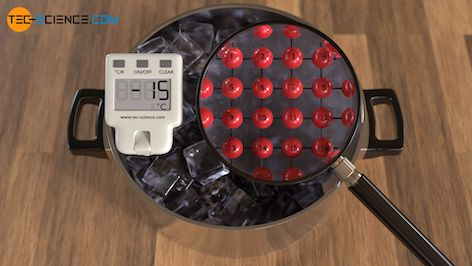
\includegraphics[trim=6.5cm 2.5cm 3.5cm 0.5cm, clip, width=0.9\textwidth]{images/aggregatzustand-fest.jpg}
    \end{flushright}
    {\scriptsize (c) \url{https://www.tec-science.com/}}\\
    {\scriptsize Modell eines Festkörpers}
\end{minipage}

%\vspace{1cm}

\textbf{Flüssigkeiten}

\begin{minipage}{0.65\textwidth}
In Flüssigkeiten wirken im Vergleich zu Feststoffen geringere Bindungskräfte, sodass die Teilchen nicht mehr an einen festen Platz gebunden sind. Die Teilchen können sich innerhalb der relativ schwach wirkenden Bindungskräfte frei bewegen und ihren Ort wechseln. Würde man die Teilchen in Gedanken nummerieren, so wäre bereits nach kurzer Zeit diese Nummerierung durcheinander. Der Stoff kann durch die geringen Bindungskräfte zwar noch zusammengehalten werden, besitzt aber aufgrund der sich frei bewegenden Teilchen keine feste Form. Eine Flüssigkeiten  passt sich jeder Gefässform an.
\vspace{0.5cm}
\end{minipage}
\begin{minipage}{0.32\textwidth}
    \begin{flushright}
        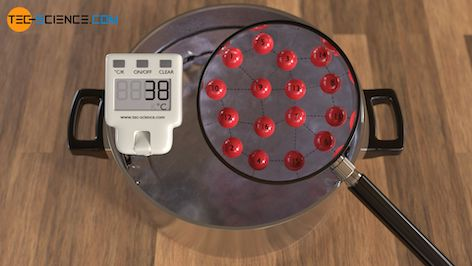
\includegraphics[trim=6.5cm 2.5cm 3.5cm 0.5cm, clip,width=0.9\textwidth]{images/aggregatzustand-fluessig.jpg}
    \end{flushright}
        {\scriptsize (c) \url{https://www.tec-science.com/}} \\
        {\scriptsize Modell einer Flüssigkeit}
\end{minipage}

%\vspace{1.2cm}


\textbf{Gase}

\begin{minipage}{0.65\textwidth}

In Gasen sind die Bindungskräfte  nochmals deutlich geringer als in Flüssigkeiten. Die einzelnen Teilchen verspüren untereinander also fast keine Bindungskräfte mehr. Sie können sich deshalb, anders als in Flüssigkeiten, relativ frei im Raum verteilen. Dies ist auch der Grund weshalb sich ein Gas den ganzen angebotenen Raum einnimmt.
\vspace{2cm}
\end{minipage}
\begin{minipage}{0.32\textwidth}
    \begin{flushright}
        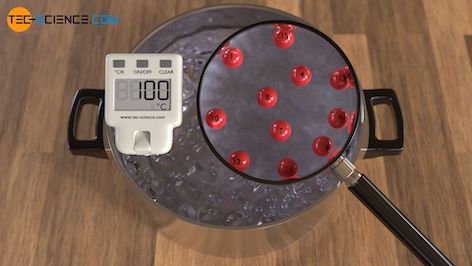
\includegraphics[trim=6.5cm 2.5cm 3.5cm 0.5cm, clip,width=0.9\textwidth]{images/aggregatzustand-gasfoermig.jpg}
    \end{flushright}
    {\scriptsize (c) \url{https://www.tec-science.com/}} \\
    {\scriptsize Modell eines Gases}

\end{minipage}

\newpage
\textbf{\Large Teilchenmodell}

Ein Stoff besteht aus kleinsten Teilchen. Das Zusammenspiel der Teilchen bestimmt die Eigenschaften. Vervollständigen Sie die folgende Tabelle mit Hilfe des Textes.

\begin{center}
    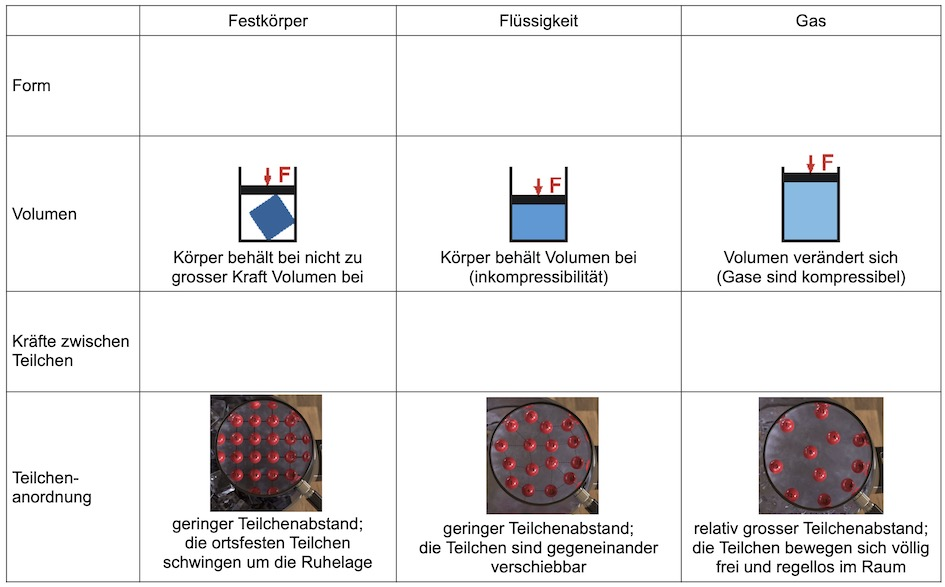
\includegraphics[width=\textwidth]{images/Tabelle.jpg}
\end{center}

\newpage

\section*{Der Druck: Definition und Einheiten}

\vspace{-0.5cm}
\begin{minipage}{0.65\textwidth}
Wenn man mit dem Finger auf einen mit Luft oder Wasser gefüllten Ballon drückt, dann kann man dies überall an den Wänden, aber auch im Inneren des Ballons nachweisen. Man sagt: ``es \underline{herrscht Druck} in der Flüssigkeit bzw. im Gas''. \\

\underline{Anders als die Kraft}, die von aussen wirkt, hat der Druck keine bestimmte Richtung – er wirkt nach allen Seiten.
\end{minipage}
\begin{minipage}{0.33\textwidth}
    \begin{flushright}
        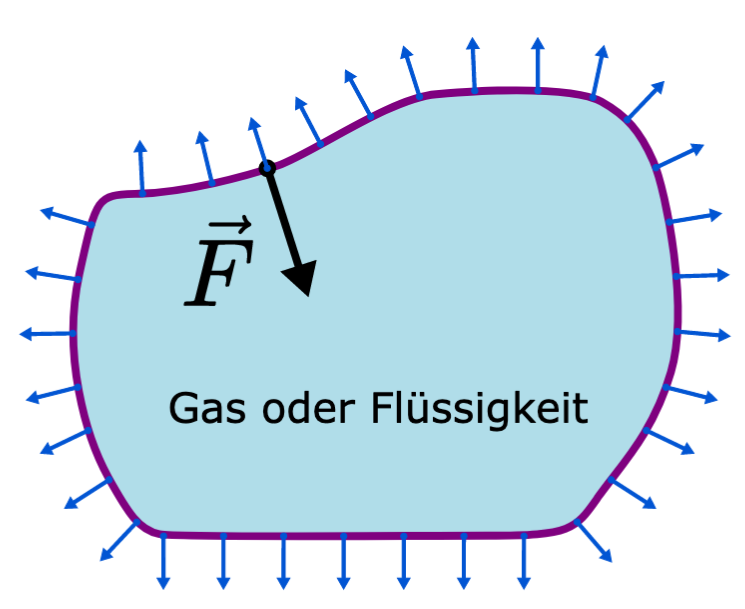
\includegraphics[width=0.95\textwidth]{images/Druck_01.png}
        {\scriptsize (c) \url{https://www.leifiphysik.de}}
    \end{flushright}
\end{minipage}


% \begin{minipage}{0.35\textwidth}
%     \begin{flushleft}
%         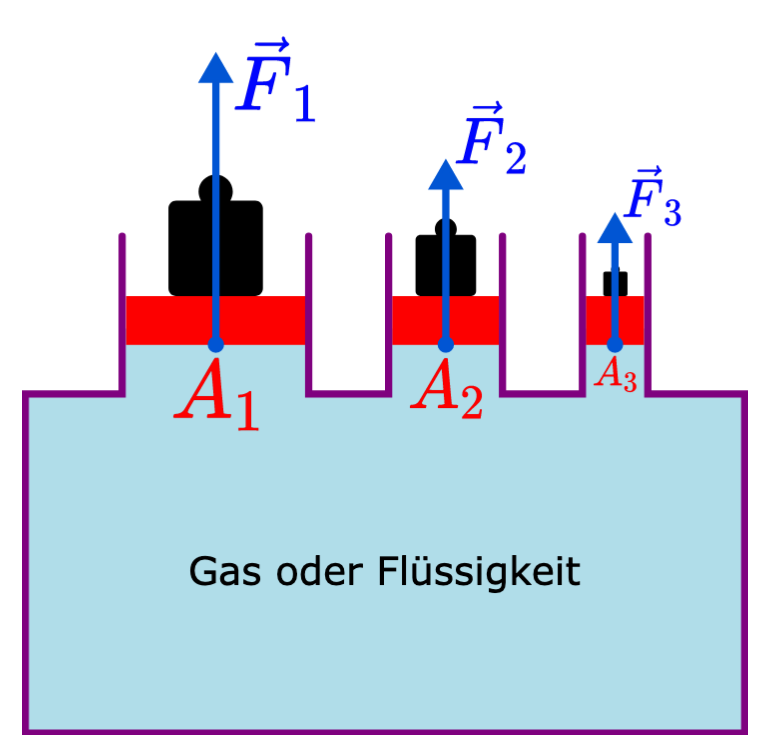
\includegraphics[width=0.95\textwidth]{images/Druck_02.png}
%         {\scriptsize (c) \url{https://www.leifiphysik.de}}
%     \end{flushleft}
% \end{minipage}
% \begin{minipage}{0.6\textwidth}


Messen können wir den Druck, indem wir feststellen, wie viel Kraft die Flüssigkeit/das Gas auf eine bestimmte Fläche ausübt. 

% Es zeigt sich, dass die Kraft der Flüssigkeit umso grösser ist, je grösser die Mess-Fläche ist. \\

Anders gesagt: Das Verhältnis aus Kraft und gedrückter Fläche ist an jeder Stelle gleich gross (\textit{die Gravitationskraft wird vernachlässigt}). Dieses Verhältnis nennen wird den Druck in der Flüssigkeit/im Gas.
% \end{minipage}






\begin{tcolorbox}[width=\textwidth, %colback=gray!10!white,colframe=gray!75!black]
    colback=white,colframe=gray!75!black]
    \textbf{Der Druck}
    
    Festlegung:  Die Grösse des Drucks kann man messen, indem bestimmt wird, wie viel Kraft auf eine bestimmte Fläche wirkt. Dann gilt

    \vspace{-0.2cm}
    $$
    p = \dfrac{F}{A}
    $$

    \vspace{-0.2cm}
    $p$ : Druck
    
    $F$ : Betrag der Kraft in N (senkrecht zur Fläche)
    
    $A$: Grösse der Fläche in $\si{\meter}^2$
    
    Die Standardmasseinheit für den Druck ist Pascal: $1\,\dfrac{\si{\N}}{\si{\meter}^2} = 1\,$Pascal $= 1\,$Pa
    
    Üblich sind die folgenden Masseinheiten:
    
    $1\,$bar $= 100\,000\,$Pa = $10^5\,Pa$ \qquad 	$1\,$mbar $= 100\,$Pa
    
    Die in den USA gebräuchliche Masseinheit des Drucks heisst ``\underline{p}ound-force per \underline{s}quare \underline{i}nch'': 
    
    $1\,$psi $\approx 6\,895\,$Pa $\approx 0.07\,$bar

\end{tcolorbox}

%\vfill
%\vspace{1cm}

\begin{minipage}{0.55\textwidth}
    \textbf{Frage:} \vspace{0.2cm}
    
    Ein Gefäss ist mit einer Flüssigkeit (einem Gas) gefüllt, wie die Abbildung zeigt. Es hat drei Öffnungen mit Kolben unterschiedlicher Fläche (A1, A3 und A3). Es herrscht Druck in der Flüssigkeit. Was können Sie anhand der Definition von Druck über die Kräfte sagen, die auf diese Kolben wirken?  Zeichnen Sie diese Kräfte. Was können Sie über die Massen sagen, die erforderlich wären, um die Kolben im Gleichgewicht zu halten?
\end{minipage}
\begin{minipage}{0.43\textwidth}
\vspace{1cm}
    \begin{flushright}
        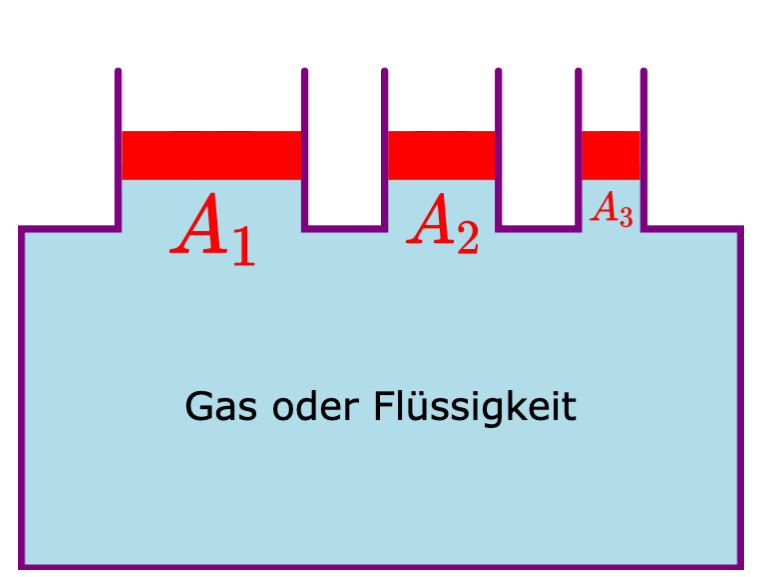
\includegraphics[width=0.95\textwidth]{images/Druck_02_Aufgabe.png}\\
        {\scriptsize (c) \url{https://www.leifiphysik.de}}
    \end{flushright}
\end{minipage}
    
\newpage

% Experiment mit hydraulischem Heber 
% Druck herrscht: Experiment mit dem Glas und Papier, umdrehen

\textbf{Rechenbeispiele}


\begin{enumerate}
    \item Sie schieben den Kolben der Velopumpe mit der Kraft 90\,N nach unten. Der Kolben hat eine Fläche von 3\,cm$^2$ . Welchen Druck zeigt das Manometer an?

    \begin{enumerate}
        \item In der Einheit Pa:\\
        \vspace{0.2cm}
        p = .........................................
        \vspace{1.5cm}

        \item In der Einheit bar:\\

	       p = .......................................
        \vspace{1.5cm}

    \end{enumerate}

    \item Der Druck in einer Sektflasche beträgt etwa 4.5\,bar. Der Flaschenhals hat einen Innendurchmesser von etwa 3\,cm. Wie viel Kraft übt das Gas in der Flasche auf den Zapfen aus? \vspace{3cm}


    \item Der Druck in einer Wasserleitung beträgt 5\,bar. Dieser Hobby-Handwerker hat aus Versehen hineingebohrt (Loch mit 5mm Durchmesser). Mit wie viel Kraft müsste er den Daumen auf die angebohrte Leitung drücken, damit kein Wasser ausfliesst? \vspace{3cm}

    \item Das abgebildete Ventil gehört zu einem Veloschlauch. Der kleine Stempel in der Mitte hat 2\,mm Durchmesser. Wenn Sie mit 3.8\,N auf den Stempel drücken müssen, um die Luft abzulassen: Wie gross ist der Druck im Schlauch? %\vspace{4cm}

    \vfill

    \hfill {\scriptsize 1) 300\,000\,Pa, 3\,bar;  2) 318\,N;    3) 9.8\,N;      4) 12\,bar }
\end{enumerate}

\newpage

\section*{Schweredruck}

\textbf{Wovon hängt der Druck ab?} Bestimmen Sie für die folgenden 5 Situationen den Druck am Boden des jeweiligen Gefässes. Die Gewichtskraft einer Flüssigkeit erhalten Sie aus der Dichte und dem Volumen. ($g\approx 10\,$m/s$^2$, $\pi \approx 3$)

\begin{figure}[h!]
    \centering
    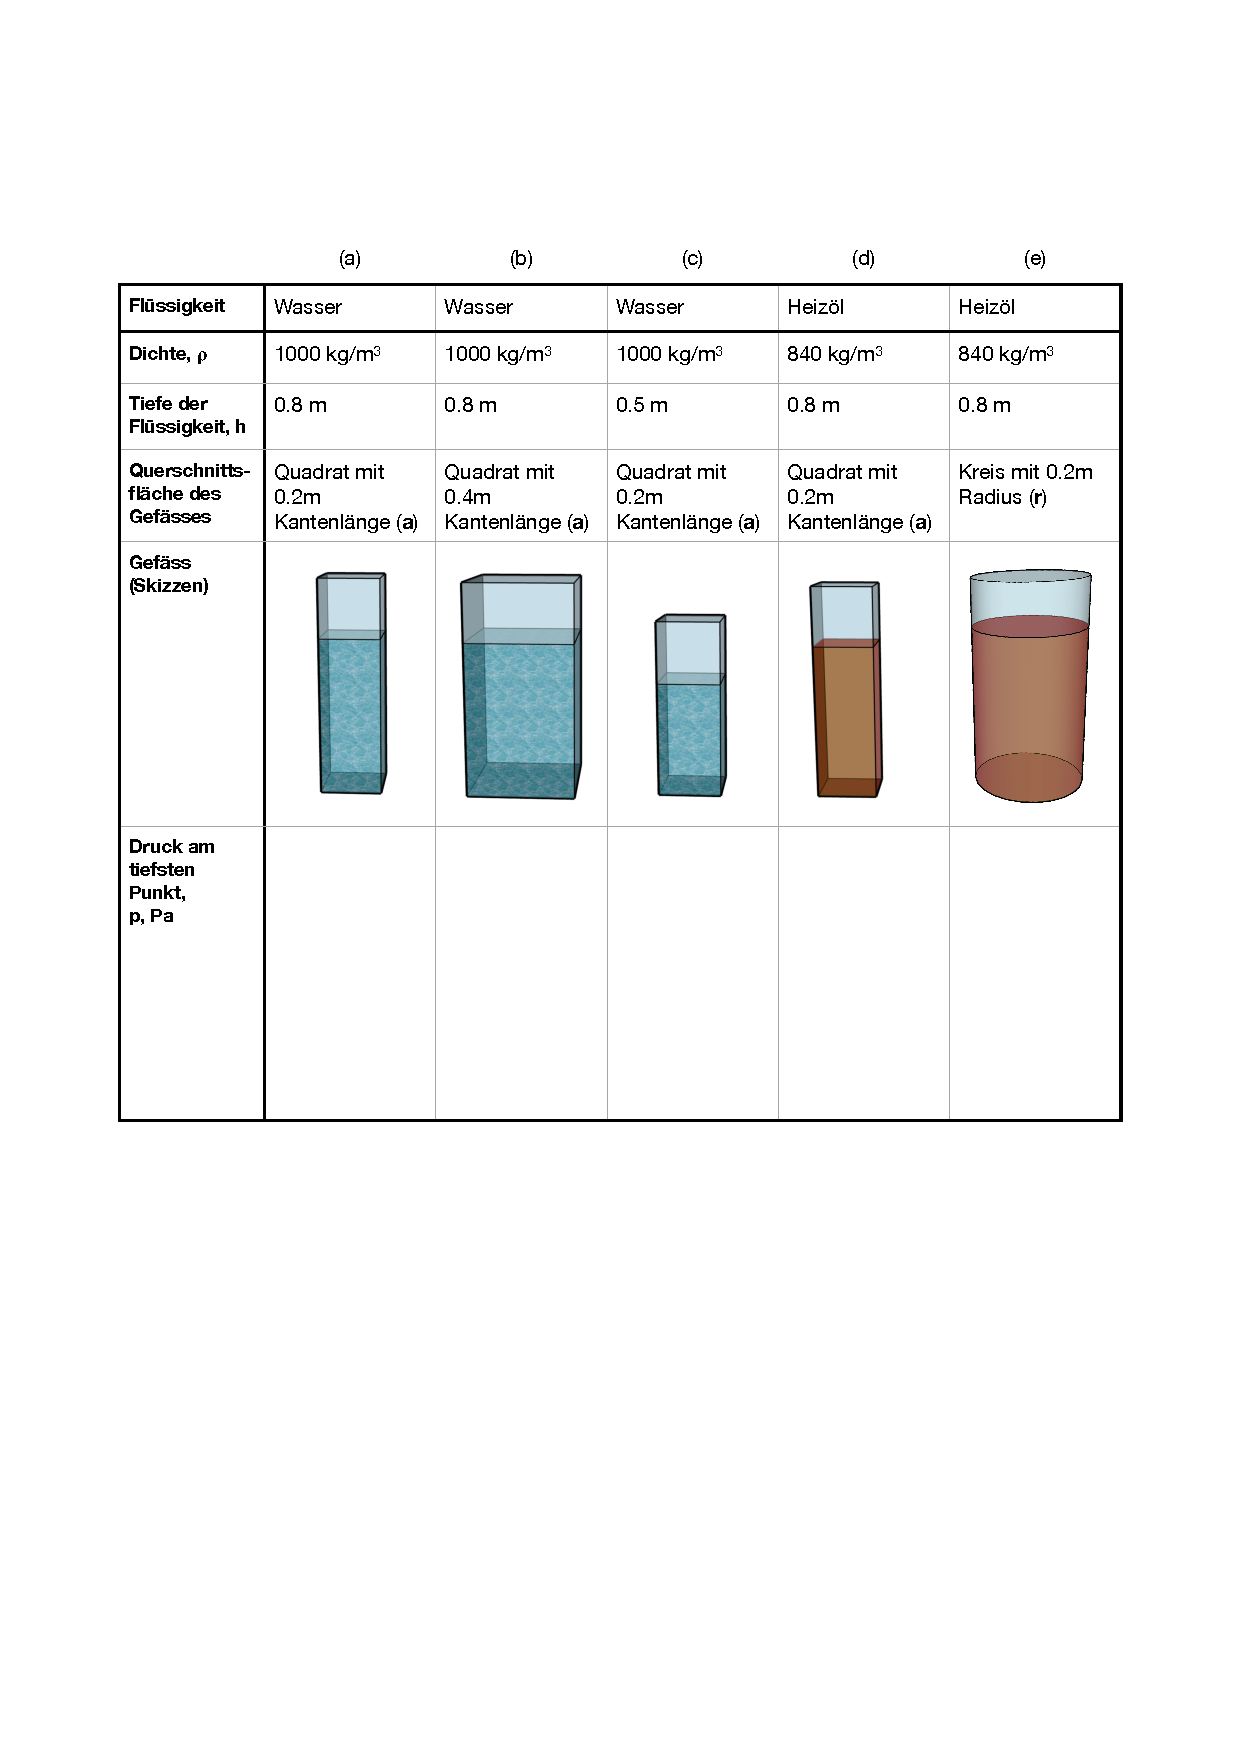
\includegraphics[width=\textwidth]{images/03_Dichte_Aufgabe.pdf}
    % \caption{Caption}
    \label{Dichte}
\end{figure}

\vfill
\textbf{Zusammenfassung}: Von welchen Grössen hängt der Druck am Boden des Gefässes \textbf{nicht} ab? \vspace{2cm}

\newpage
\textbf{Gleichung für Schweredruck}

Leiten Sie eine allgemeine Formel für den Druck her. \textit{(Hinweis: Fängen Sie mit der Gleichung für den Druck an. Benutzen Sie dann die Gleichungen der Gewichtskraft und der Dichte.)}

\vspace{7cm}

\textbf{Beispiele}
\vspace{-0.3cm}


\begin{enumerate}

    % \begin{wrapfigure}[5]{r}{0.3\textwidth}
    %     \centering
    %     \vspace{-0.5cm}
    %     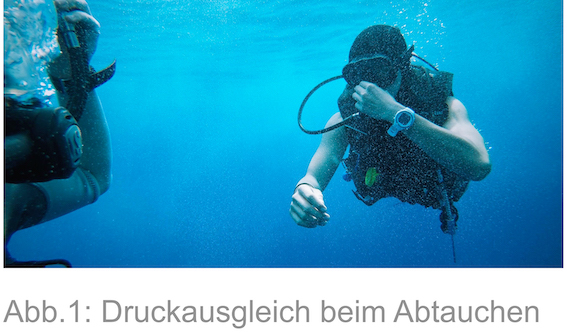
\includegraphics[width=\linewidth]{images/Taucherregel.jpg}
    %     %\caption{Caption}
    %     %\label{fig:wrapfig}
    % \end{wrapfigure}
    

    \item Die Taucherregel laut: Pro 10 Meter Wassertiefe steigt der Druck um 1\,bar. Überprüfen Sie diese Regel. ($g \approx 10\,$N/kg, $\rho_{Waser} \approx 1000\,$kg/m$^3$) 

    \begin{figure}[h!]
    \begin{flushright}
        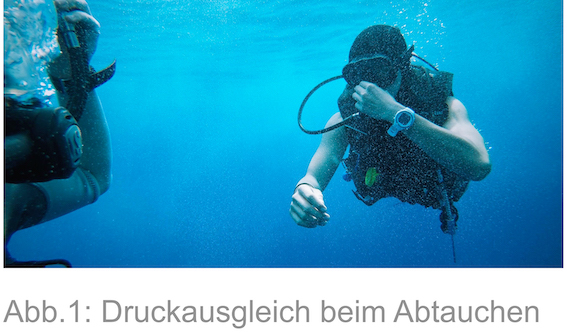
\includegraphics[width=0.25\textwidth]{images/Taucherregel.jpg}
        %\caption{Caption}
        \label{fig:Taucher}        
    \end{flushright}
    \end{figure}
    
    \vspace{-1cm}

    Ergänzen Sie die Skizze mit Hilfe dieser Taucherregel. Welcher Druck herrscht in verschiedenen Tiefen?

    \vspace{0.3cm}

    \begin{figure}[h!]
    \begin{flushright}
        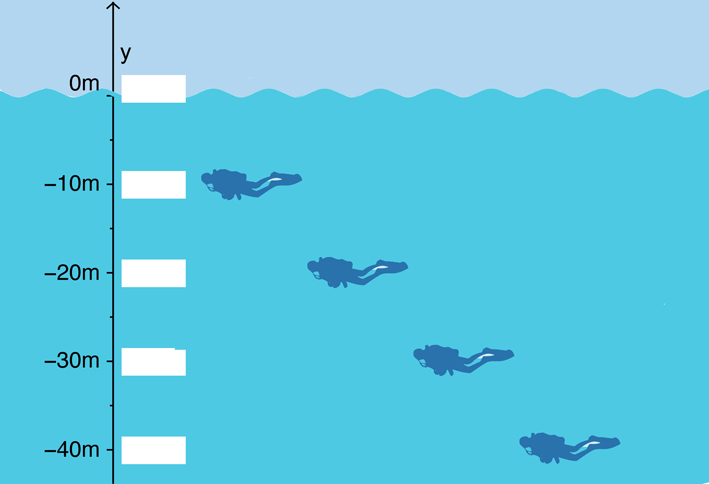
\includegraphics[width=0.6\textwidth]{images/Meer_Tiefe.jpg}
        %\caption{Caption}
        \label{fig:regel}        
    \end{flushright}
    \end{figure}

    \newpage
    \begin{minipage}{0.5\textwidth}
    \item 
    \begin{enumerate}
        \item Welcher Druck herrscht in 11000 m Meerestiefe? ($g \approx 10\,$N/kg, Salzwasser: Dichte $1.030\,$g/cm$^3$)

        \item Wie gross ist dort die Kraft auf die aussen Seite vom Fenster? (äussere Durchmesser 40\,cm)
        \item Welcher Masse in Tonnen entspricht diese Kraft?
        
    \end{enumerate} 
    \end{minipage}
    \begin{minipage}{0.45\textwidth}
        \begin{flushright}
            % trim: left bottom right top
            %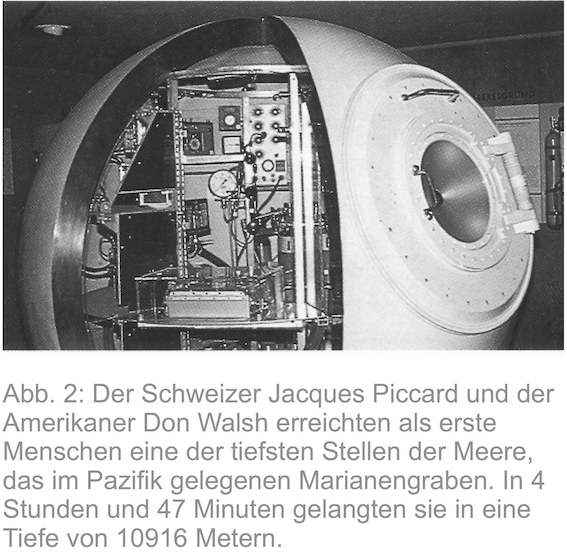
\includegraphics[trim=0cm 2.5cm 0cm 0cm, clip, width=0.9\textwidth]{images/Marianengraben.jpg}
    
            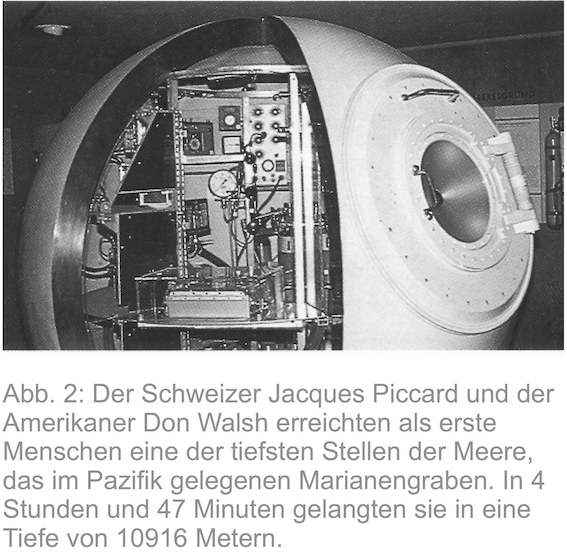
\includegraphics[width=0.9\textwidth]{images/Marianengraben.jpg}
    
            % \begin{flushleft}
                %  {\footnotesize Der Schweizer Jacques Piccard und der Amerikaner Don Walsh erreichten als erste Menschen eine der tiefsten Stellen der Meere, das im Pazifik gelegenen Marianengraben. In 4 Stunden und 47 Minuten gelangten sie in eine Tiefe von 10\,916\, Metern.}
            % \end{flushleft}
            

        \end{flushright}
    \end{minipage}
    
\end{enumerate}

% mehr über die Idee von Piccard

% Lösung
% 
%\begin{enumerate}[label=(\alph*)]
%     \item $p = \rho g  h \approx 1030\,\si{\kg}/\si{\meter}^3 \cdot 10\,\si{\meter}/\si{\second}^2 \cdot 11000\,\si{\meter} \approx 1.13\times 10^8\,\si{\pascal}$
%     \item $F = p\cdot A = 1.13\times 10^8\,\si{\pascal} \cdot (\pi \cdot (0.2\,\si{\meter})^2) \approx 1.4 \times 10^7\,\si{\N}$
%     \item $m = \dfrac{F}{g} = \dfrac{1.4 \times 10^7\,\si{\N}}{10\,\si{\meter}/\si{\second}^2 } \approx 1400$\,Tonnen
% \end{enumerate}


\newpage

\section*{Hydrostatisches Paradoxon}


\textbf{Experiment}: 
Verschiedene Gefässe mit gleicher Grundfläche werden mit Wasser gefühlt. Die Kraft, die das Wasser auf die Membran ausübt, wird mit dem Zeiger angezeigt.

 \textbf{Frage}: Wie viel Wasser passt in jedes Gefäss, wenn der Zeiger die gleiche Kraft anzeigt, die auf die Membran wirkt?

\textbf{Vermutung}: 
    %\vspace{0.5cm}

\begin{center}
    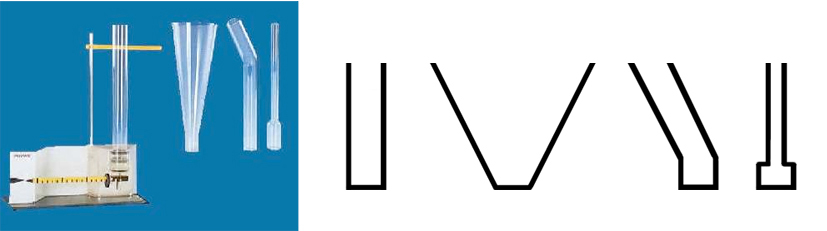
\includegraphics[width=0.8\textwidth]{images/Experiment_hight.jpg}
\end{center}

\textbf{Beobachtung}: 
    \vspace{1cm}

\begin{tcolorbox}[width=\textwidth, %colback=gray!10!white,colframe=gray!75!black]
        colback=white,colframe=gray!75!black]
        \textbf{Hydrostatisches Paradoxon}
        \vspace{1.5cm}
\end{tcolorbox}

\vspace{0.5cm}

Weitere Beispiele:
\begin{center}
    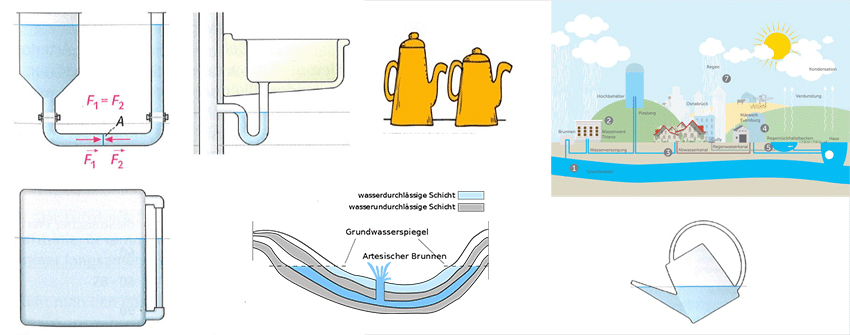
\includegraphics[width=0.9\textwidth]{images/Beispiele_hydroParadoxon.jpg}
\end{center}

\newpage

\begin{minipage}{0.7\textwidth}
    \textbf{Fassversuch von Pascal}: Blaise Pascal (1623 – 1662), so wird erzählt, hat einmal in einer Gesellschaft behauptet, er könne mit wenigen Gläsern Rotwein ein volles Weinfass zum Bersten bringen. Da ihm das niemand glaubte, führte er folgendes vor:

    Er nahm ein langes dünnes Rohr. Dieses stellte er senkrecht auf, so dass es mehrere Meter in die Höhe ragte. Das untere Ende des Rohrs steckte er in das Fass. Nachdem alle Öffnungen abgedichtet waren, füllte er das Rohr mit Rotwein. Weil das Rohr dünn war, genügten hierfür wenige Gläser. Während des Auffüllens begann das Fass plötzlich zu krachen und zerbarst in mehrere Teile.

    \begin{enumerate}
        \item Angenommen, das Rohr war bis in 10\,m Höhe mit Wein (= Wasser) gefüllt: Wie viel Kraft übte der Wein auf ein Brett des Fasses aus (Fläche eines Brettes: 15\,cm x 40\,cm). \vspace{3cm}
        
        \item Welcher Masse in Kilogramm entspricht diese Kraft?
    \end{enumerate}

\end{minipage}
\begin{minipage}{0.28\textwidth}
    \begin{flushright}
        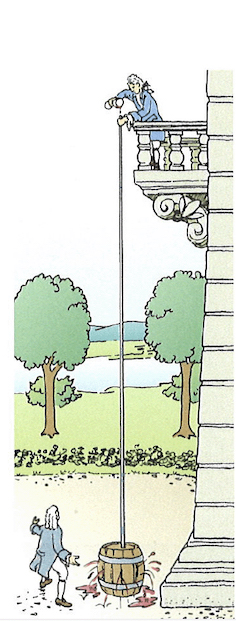
\includegraphics[width=0.9\textwidth]{images/Pascal.jpg}
    \end{flushright}
\end{minipage}

% kommunizierende Rohre: Experiment mit Schlauch, etwas ausleeren > Der Becher von Pythagoras


\vspace{5cm}

\textbf{Der Becher des Pythagoras (Becher der Gerechtigkeit)}
\begin{flushleft}
    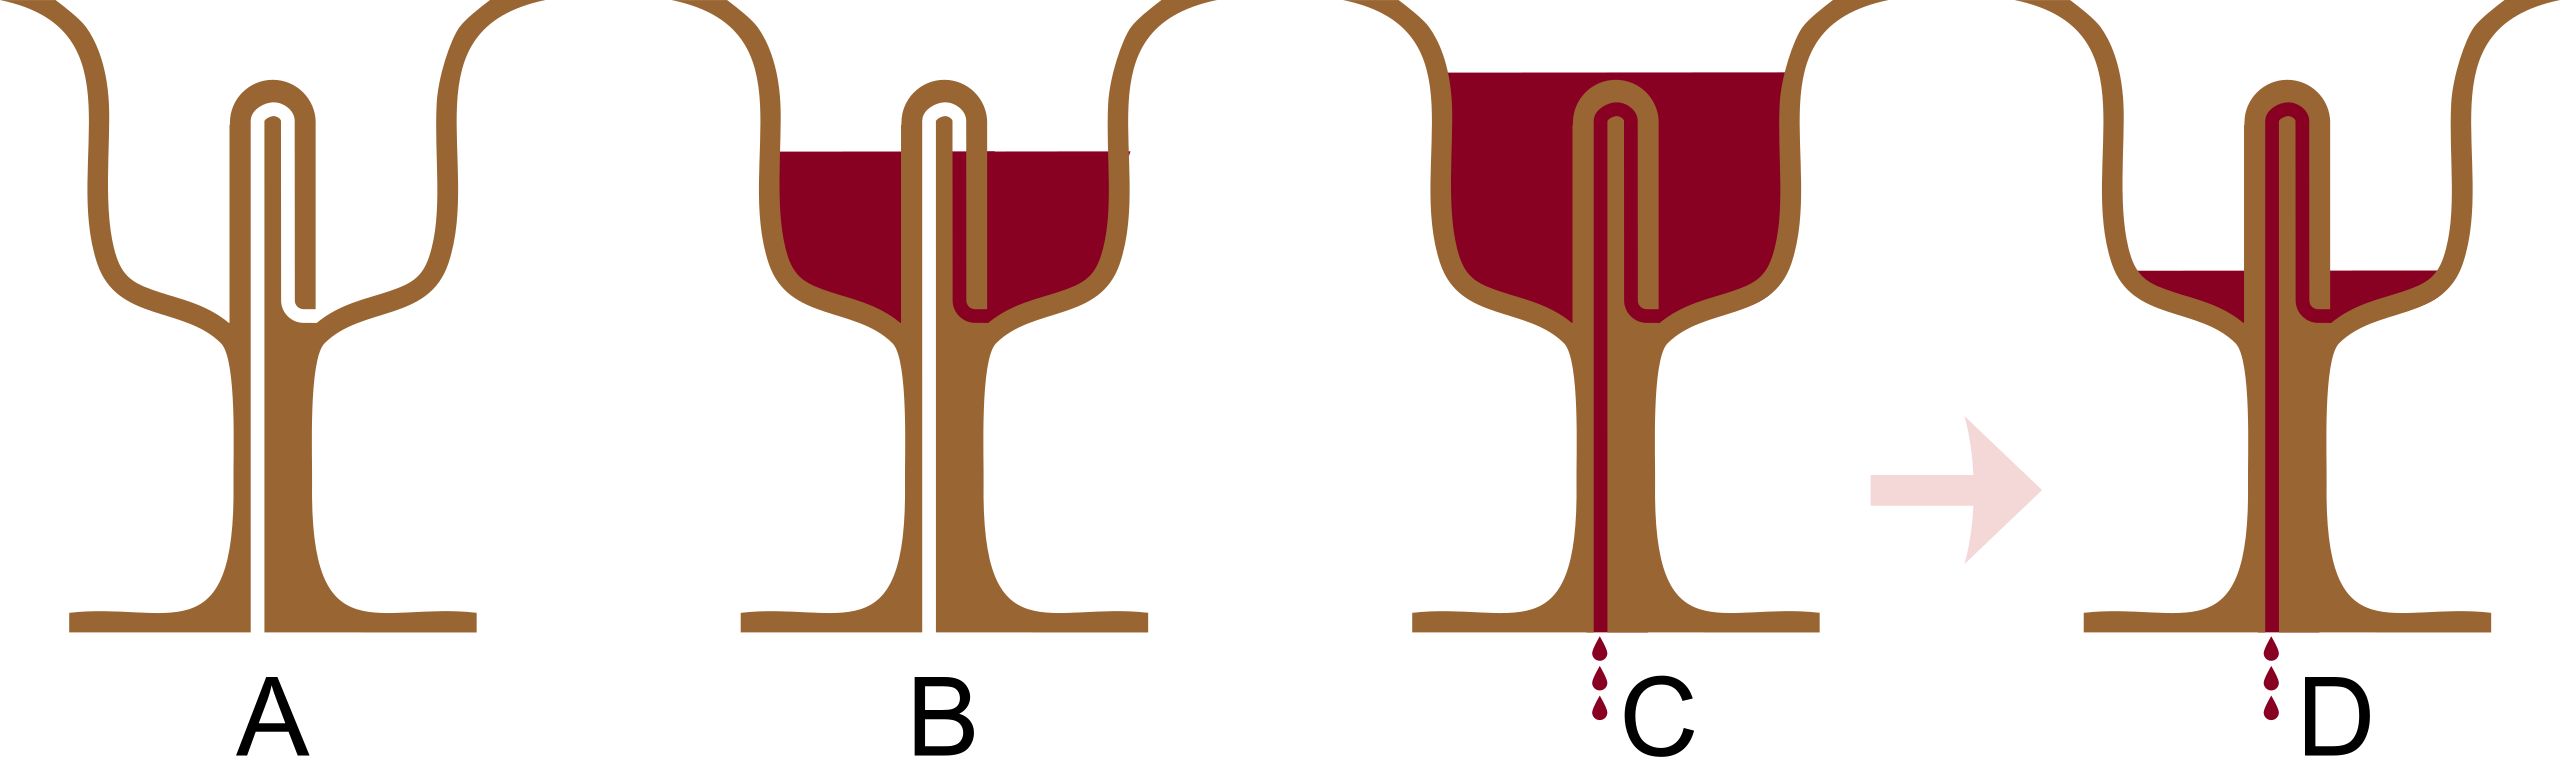
\includegraphics[width=0.75\textwidth]{images/Physagorian_Pythagoras.png}
\end{flushleft}

% Kommunizierende Röhren, Druckdifferenz,  [Ein Heber, Saugheber, Winkelheber]

% Das Fliessen in der vollständig mit Flüssigkeit gefüllten Leitung erfolgt aufgrund dieser Druckdifferenz nach dem Prinzip der kommunizierenden Röhren. 

% stabil: Das System kehrt nach einer Störung wieder in seinen Ausgangszustand zurück.

% labil: Das System geht bei der kleinsten Störung in einen anderen Zustand über.


\newpage

% Einstieg mit der Knetmasse 
% Einstieg mit den Folien/Beispielen

\section*{Der hydrostatische Auftrieb}

\begin{figure}[h!]
    \centering
    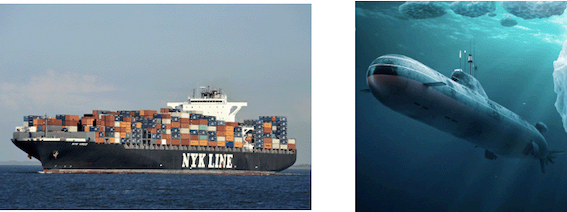
\includegraphics[width=0.6\textwidth]{images/Auftrieb_Schiff_UBoot.jpg}
\end{figure}

Warum kann ein grosses, schweres Schiff schwimmen? Wie sinken und steigen U-Boote? 
\\Warum schwimmen manche Gegenstände und andere sinken?

Diese und andere Fragen können werden nach dieser Lektion beantwortet.

\subsection*{Einführung}

%Der \textbf{hydrostatische Auftrieb} im Wasser entsteht durch den Unterschied im hydrostatischen Druck in einer Flüssigkeit.

\textbf{Versuch} mit Knetmasse 

In diesem Versuch können wir bereits erste Erkenntnisse darüber gewinnen, wie Flüssigkeit (Wasser) das Gewicht von Körpern verändert. 

\textbf{Skizze}

\begin{tikzpicture}
    \draw[step=5mm, line width=0.2mm, black!20!white] (0,0) grid  (17cm, 5.5cm);% 10cm);
\end{tikzpicture}


\textbf{Notizen}

\begin{tikzpicture}
    \draw[step=5mm, line width=0.2mm, black!20!white] (0,0) grid  (17cm, 2cm);% 10cm);
\end{tikzpicture}

\textbf{Vermutung: }Was hat sich geändert?

\begin{tikzpicture}
    \draw[step=5mm, line width=0.2mm, black!20!white] (0,0) grid  (17cm, 2cm);% 10cm);
\end{tikzpicture}

\newpage

\subsection*{Herleitung: Auftriebskraft}

\begin{minipage}{0.75\textwidth}
    \textbf{Aufgabe 1}: Das Gefäss rechts ist mit Wasser gefüllt. Ordnen Sie die Punkte A, B, C, D nach dem Druckanstieg.\vspace{4cm}

\end{minipage}
\begin{minipage}{0.25\textwidth}
    \begin{flushright}
        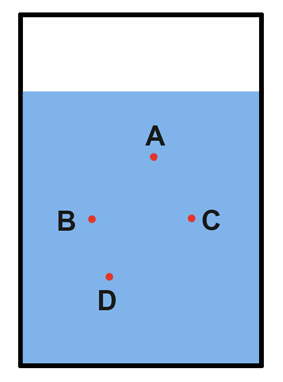
\includegraphics[width=0.95\textwidth]{images/Auftrieb_A1.png}
    \end{flushright}
\end{minipage}

\begin{minipage}{0.65\textwidth}
    \vspace{-1cm}
    \textbf{Aufgabe 2}: Nun tauchen wir einen Zylinders ins Wasser. 
    \begin{enumerate}[label=(\alph*)]
        \item Vergleichen Sie den Druck an der Ober- und Unterseite des Zylinders. \vspace{1cm}
        \item Vergleichen Sie den Druck auf der linken und rechten Seite des Zylinders. \vspace{1cm}
        \item Zeichnen Sie jetzt an den markierten Stellen (1-4) ein, welche Kräfte auf jede der Seiten des Zylinders wirken.
    \end{enumerate}
\end{minipage}
\begin{minipage}{0.35\textwidth}
    \begin{flushright}
        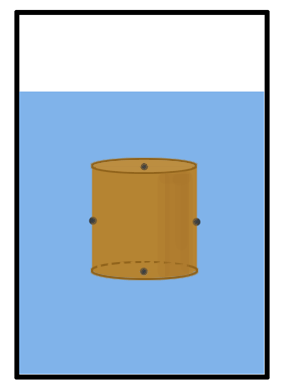
\includegraphics[width=0.9\textwidth]{images/Auftrieb_A2.png}
    \end{flushright}
\end{minipage}
\vspace{1cm}

\textit{Hinweise:
\begin{itemize}
    \item Der Druck hat bekanntlich keine Richtung (es herrscht Druck). Sobald wir aber eine bestimmte Fläche eines Gegenstandes betrachten, der diesem Druck ausgesetzt ist, können wir die Kraft angeben, die auf diese Fläche ausgeübt wird. Diese Kraft wirkt senkrecht auf die Fläche.
    \item Die Länge der Pfeil entspricht dem Betraf einer Kraft.
    %\item Erinnerung: Die Kraft kann durch den hydrostatischen Druck, oder Schweredruck bestimmt werden: $F = A \cdot p$, wobei $p = \rho_F \cdot g \cdot h$.
\end{itemize}
}

\begin{enumerate}
    \item [(d)] Wie gross ist die resultierende Kraft, die auf diesen Zylinder einwirkt? Muss man alle Kräfte berücksichtigen?
\end{enumerate}


\newpage
\subsection*{Formale Herleitung der Auftriebskraft}

\begin{minipage}{0.65\textwidth}
Verwenden Sie bei der Herleitung folgene Bezeichnungen:
\begin{itemize}
    \item $A$ - Seitenfläche des Zylinders
    \item $h$ - Höhe des Zylinders
    \item $h_1$ - Tiefe bis zur oberen Fläche
    \item $h_2$ - Tiefe bis zu unteren Fläche 
    \item $\rho_F$ - Dichte der Flüssigkeit
\end{itemize}
% \begin{tabular}[r l]
%     A & Seitenfläche des Zylinders \\
%     h & Höhe des Zylinders \\
%  %   $h_1$    & Tiefe bis zur oberen Fläche \\
%  %   $h_2$    & Tiefe bis zu unteren Fläche \\
%  %   $\rho_F$ & Dichte der Flüssigkeit \\
% \end{tabular}
\end{minipage}
\begin{minipage}{0.35\textwidth}
    \begin{flushright}
        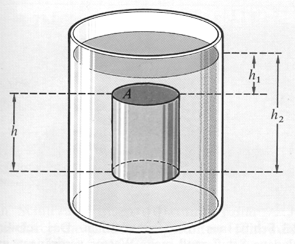
\includegraphics[width=0.9\textwidth]{images/Herleitung_Auftrieb_bw.png}
    \end{flushright}
\end{minipage}

Bestimmen Sie formal (nur mit Buchstaben) die folgenden Grössen. 

den Druck an der oberen Zylinderfläche: \\
$p_1 =$ \vspace{0.5cm} 

die Kraft auf die obere Zylinderfläche: \\
$F_1 = $ \vspace{0.5cm}

den Druck an der unteren Zylinderfläche: \\
$p_2 = $ \vspace{0.5cm}

die Kraft auf die untere Zylinderfläche: \\
$F_2 = $ \vspace{0.5cm}


Die Auftriebskraftraft ist die Differenz zwischen den Kräften $F_2$ und $F_1$ 
\vspace{3cm}


\begin{tcolorbox}[width=\textwidth, %colback=gray!10!white,colframe=gray!75!black]
    colback=white,colframe=gray!75!black]
    \textbf{Auftrieb (Auftriebskraft)}
    \vspace{3cm}
\end{tcolorbox}

\newpage
\subsection*{Archimedisches Prinzip}

%Scheinbare Gewicht von einem Körper, der in eine Flüssigkeit getaucht wird, hängt von der Auftriebskraft ab. Man kann folgende Fälle unterscheiden: Körper sinkt, Körper schwebt, Körper schwimmt (steigt). 
Anhand der Auftriebskraft lassen sich die folgenden Fälle unterscheiden: Der Körper sinkt, der Körper schwebt, der Körper schwimmt (Bewegung zur Oberfläche). Können Sie die Regeln definieren, indem Sie die Gewichtskraft ($F_G$) und die Auftriebskraft ($F_A$) vergleichen?

\hspace{1.5cm} sinken \hspace{4cm} schweben \hspace{4cm} schwimmen

\vspace{3cm}

\begin{tcolorbox}[width=\textwidth, %colback=gray!10!white,colframe=gray!75!black]
    colback=white,colframe=gray!75!black]
    \textbf{Archimedisches Prinzip}
    \begin{flushright}
        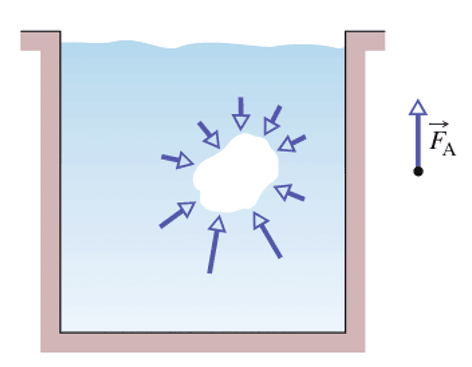
\includegraphics[width=0.3\textwidth]{images/Archimedisches_Prinzip.png}
    \end{flushright}

    \vspace{1cm}
\end{tcolorbox}



\newpage

% Platz für Experiment "Archimedischer Zylinder machen"
\textbf{Beispiel: Eiswürfel}

\begin{minipage}{0.8\textwidth}
Ein Eiswürfel mit der Kantenlänge 2\,cm schwimmt in einem Glas Wasser.

	$g = 9.81\,$N/kg\\
	$\rho_{Wasser} = 1000\,$kg/m$^3$ \\
	$\rho_{Eis} = 917\,$kg/m$^3$
\end{minipage}
\begin{minipage}{0.2\textwidth}
    \begin{flushright}
        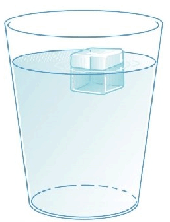
\includegraphics[width=0.8\textwidth]{images/Beispiel-Eis.png}
    \end{flushright}

    % Für einen Körper, der sich in einer Flüssigkeit oder in einem Gas befindet, gilt: die auf den Körper wirkende Auftriebskraft ist gleich der Gewichtskraft der von ihm verdrängten Flüssigkeits- bzw. Gasmenge.
\end{minipage}

\begin{enumerate}[label=(\alph*)]
    \vspace{-0.5cm}
    \item Wie gross ist die Gewichtskraft, die auf den Eiswürfel wirkt? \vspace{2cm}
    
    \item Sie üben so viel Kraft aus, dass der ganze Würfel gerade unter Wasser ist. Wie gross ist die Auftriebskraft, die auf die Eiswürfel wirkt? Vergleichen Sie diese Auftriebskraft mit der Gewichtskraft. \vspace{2cm}
    
    \item Wenn Sie nun den Eiswürfel loslassen, würde ein Teil von ihm wieder über der Wasseroberfläche erscheinen. Ohne zusätzliche Kraft schwebt der Eiswürfel im Wasser. Welche Auftriebskraft wirkt jetzt auf den Eiswürfel? \vspace{2cm}

    \item Welchem verdrängten Wasservolumen entspricht diese Auftriebskraft? \vspace{2cm}

    \item Angenommen, der Eiswürfel schwimmt perfekt senkrecht, so dass seine Unter- und Oberseite parallel zur Wasseroberfläche sind. Wie viel von der Höhe des Eiswürfels befindet sich oberhalb der Wasseroberfläche?
\end{enumerate}


%*****************************Lösungen
\newpage
\textbf{Beispiel: Eiswürfel}

\begin{minipage}{0.8\textwidth}
Ein Eiswürfel mit der Kantenlänge 2\,cm schwimmt in einem Glas Wasser.

	$g = 9.81\,$N/kg\\
	$\rho_{Wasser} = 1000\,$kg/m$^3$ \\
	$\rho_{Eis} = 917\,$kg/m$^3$
\end{minipage}
\begin{minipage}{0.2\textwidth}
    \begin{flushright}
        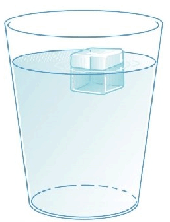
\includegraphics[width=0.8\textwidth]{images/Beispiel-Eis.png}
    \end{flushright}
\end{minipage}

\begin{enumerate}[label=(\alph*)]
    \vspace{-0.5cm}
    \item Wie gross ist die Gewichtskraft, die auf den Eiswürfel wirkt? 
    
    \color{OliveGreen}
    $F_g = m_{Eis}g = \rho_{Eis} \cdot V_{Eis} \cdot g \approx 0.072\,N$
    \vspace{1cm}
    
    \color{black}
    \item Sie üben so viel Kraft aus, dass der ganze Würfel gerade unter Wasser ist. Wie gross ist die Auftriebskraft, die auf die Eiswürfel wirkt? Vergleichen Sie diese Auftriebskraft mit der Gewichtskraft. 
    
    \color{OliveGreen}
    $F_A = \rho_{Wasser} \cdot V_{Eis} \cdot g \approx 0.078\,N$
    \color{black}
    \vspace{0.5cm}
    
    \item Wenn Sie nun den Eiswürfel loslassen, würde ein Teil von ihm wieder über der Wasseroberfläche erscheinen. Ohne zusätzliche Kraft schwebt der Eiswürfel im Wasser. Welche Auftriebskraft wirkt jetzt auf den Eiswürfel? 
    
    \color{OliveGreen}
    Die $F_A$ ist genau so gross wie die $F_g$.
    \color{black}
    \vspace{0.5cm}

    \item Welchem verdrängten Wasservolumen entspricht diese Auftriebskraft? 
    
    \color{OliveGreen}
    $F_A = 0.072\,N$ \\ \vspace{0.5cm}
    $V_{verdr} = \dfrac{F_A}{\rho_Wasser \cdot g} \approx 7.3\times 10^{-6}\,$m$^3 = 7.3\,$cm$^3$
    \color{black}


    \item Angenommen, der Eiswürfel schwimmt perfekt senkrecht, so dass seine Unter- und Oberseite parallel zur Wasseroberfläche sind. Wie viel von der Höhe des Eiswürfels befindet sich oberhalb der Wasseroberfläche?
    
    \color{OliveGreen}
    $h_{unterhalb} = \dfrac{V_{verdr}}{A_{Eis}} \approx 1.825\,$cm

    $h_{oberhalb} = 0.175\,$cm

    \color{black}
    
    \item Wie viel zusätzliche Masse kann auf die Eiswürfel aufgeladen werden, sodass seine Oberseite sich genau auf der Wasseroberfläche befindet? 

    \color{OliveGreen}
    $F_{g,zu} = F_{A,voll} - F_g = 0.006\,N$
    
    Das entspricht der Masse: $m = \dfrac{F_{g,zu}}{g} \approx 0.06\,$g 
    \color{black}


    
    \item Wie ändert sich die Auftriebskraft, wenn Sie die Eiswürfel tiefer hineindrücken? Warum?

    \color{OliveGreen}
    Die $F_A$ ändert sich nicht. Bei der Auftriebskraft geht es um den Höhenunterschied. 
    \color{black}

\end{enumerate}
%*************************************


\end{document}
